\documentclass{standalone}
\usepackage{graphicx}	
\usepackage{amssymb, amsmath}
\usepackage{color}

\usepackage{tikz}
\usetikzlibrary{intersections, backgrounds, math}
\usepackage{pgfmath}

\definecolor{light}{RGB}{220, 188, 188}
\definecolor{mid}{RGB}{185, 124, 124}
\definecolor{dark}{RGB}{143, 39, 39}
\definecolor{highlight}{RGB}{180, 31, 180}
\definecolor{gray10}{gray}{0.1}
\definecolor{gray20}{gray}{0.2}
\definecolor{gray30}{gray}{0.3}
\definecolor{gray40}{gray}{0.4}
\definecolor{gray60}{gray}{0.6}
\definecolor{gray70}{gray}{0.7}
\definecolor{gray80}{gray}{0.8}
\definecolor{gray90}{gray}{0.9}
\definecolor{gray95}{gray}{0.95}


\begin{document}

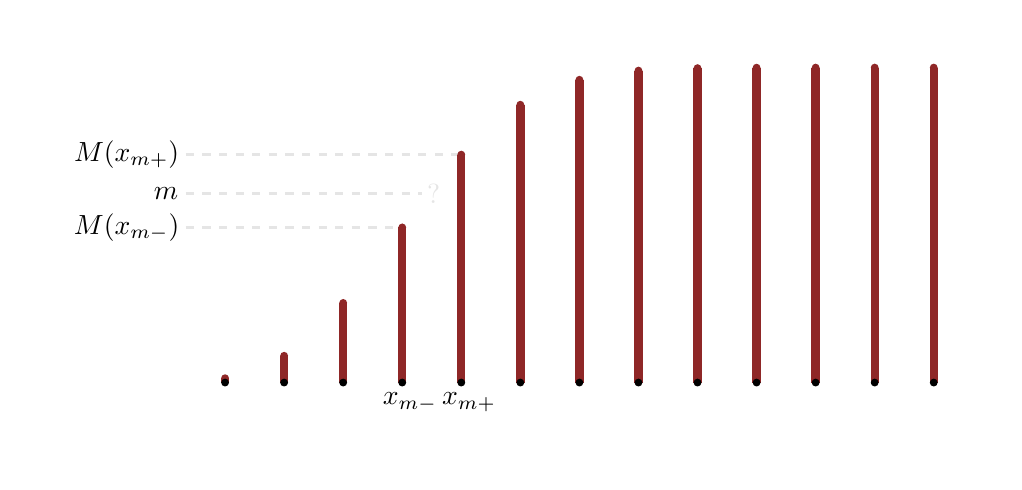
\begin{tikzpicture}[scale=1]
  \begin{scope}[shift={(0, 0)}]
    \draw[white] (-7, -3) rectangle (5.25, 2.5);
    
    \draw[gray90, dashed, line width=1] (-5, {4 * 0.6 - 2}) -- (-2, {4 * 0.6 - 2});
    \node[gray90] at (-1.85, {4 * 0.6 - 2}) { $?$ };
    \node at (-5.25, {4 * 0.6 - 2}) { $m$ };
    
    \draw[gray90, dashed, line width=1] (-5, {4 * 0.492516 - 2}) -- (-2.25, {4 * 0.492516 - 2});
    \node at (-5.75, {4 * 0.492516 - 2}) { $M(x_{m-})$ };
    
    \draw[gray90, dashed, line width=1] (-5, {4 * 0.723655 - 2}) -- (-1.5, {4 * 0.723655 - 2});
    \node at (-5.75, {4 * 0.723655 - 2}) { $M(x_{m+})$ };
    
    \foreach [count=\n] \m in {0.013841, 0.085025, 0.252815, 0.492516, 0.723655, 0.882151, 0.961399, 0.990511, 0.998308, 0.999794, 0.999985, 0.999999, 1.000000} {
      \pgfmathsetmacro{\x}{0.75 * ( (\n - 1) - 6)};
      \draw[dark, line width=3] (\x, -2) -- (\x, {(4 * \m - 2)});
      \fill[dark] (\x, {(4 * \m - 2)}) circle (0.05);
      \fill[black] (\x, -2) circle (0.05);
    }
      
    \node at (-2.25, -2.25) { $\;\; x_{m-}$ };
    \node at (-1.5, -2.25) { $\;\; x_{m+}$ };
  \end{scope}
  
\end{tikzpicture}

\end{document}  